% =============================================================================
% Appendix: Supplementary Material
% =============================================================================
% SPDX-FileCopyrightText: 2026 Frank Langbein <frank@langbein.org>
% SPDX-License-Identifier: LPPL-1.3c
%
% Appendices hold supporting material (detailed tables, derivations, survey text,
% user-study materials) so the main narrative stays focused. Complete source
% code is usually submitted separately, not in the report. Use \chapter and
% \section as in main chapters. Replace with your own supplementary material.
% =============================================================================

This appendix contains supplementary material like tables containing raw data

\section{Additional tables}\label{app:tables}

\subsection{Label Mapping and Semantics}\label{app:semantics}

\begin{table}[H]
\centering
\caption{Semantic Label Mapping Rules}
\label{tab:label_mapping}
\begin{tabular}{ll | ll}
\toprule
\textbf{Original Label} & \textbf{Mapped Class} & \textbf{Substring Rule} & \textbf{Mapped Class} \\ \midrule
table\_and\_chairs      & Table                 & 'chair'                 & Chair                 \\
office\_chair           & Chair                 & 'computer'              & Appliance             \\
hangout\_chair          & Chair                 & 'whiteboard'            & Wall\_Decoration      \\
office\_box             & Storage               & 'toilet'                & Thing                 \\
mini\_fridge            & Appliance             & 'wastebasket'           & Storage               \\
reception\_desk         & Table                 & 'desk'                  & Table                 \\
corner                  & Structure             & 'monitor'               & Appliance             \\ 
\bottomrule
\end{tabular}
\end{table}


\begin{figure}[H]
    \centering
    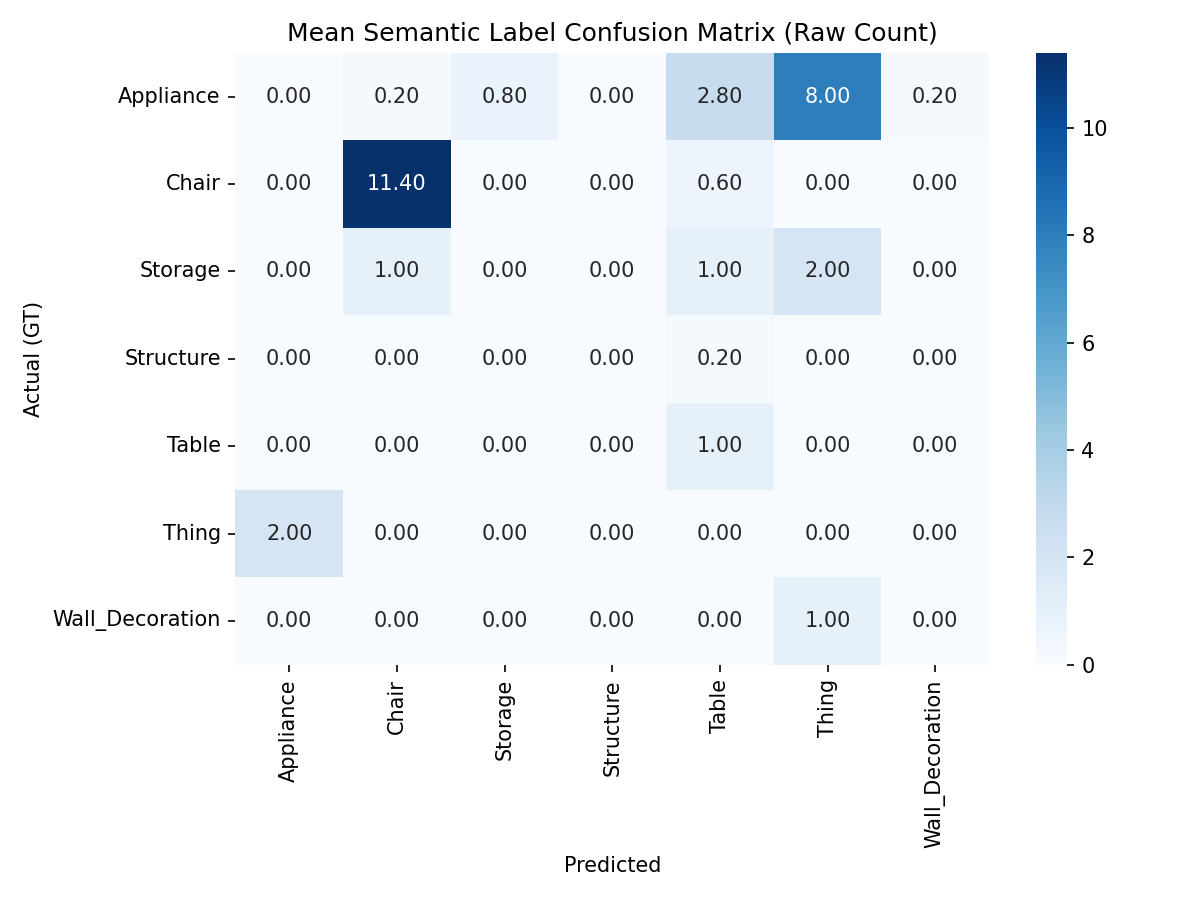
\includegraphics[width=0.9\textwidth]{figures/confusion_matrix_mean_raw.png}
    \caption{Mean Count Confusion Matrix of Hydra Labels vs Ground Truth Labels}
    \label{fig:app:semantics:hydra_cmatrix}
\end{figure}

\subsection{Room Recognition Per-Run}\label{app:room-recognition}

\begin{table}[H]
\centering
\caption{Raw Room Recognition Results over 5 Evaluation Runs}
\label{tab:raw_room_results}
\begin{tabular}{l | ccc | ccc | ccc}
\toprule
\textbf{Run} & \multicolumn{3}{c|}{\textbf{S-Graphs+}} & \multicolumn{3}{c|}{\textbf{Hydra}} & \multicolumn{3}{c}{\textbf{Clio}} \\ 
 & Recall & Precision & F1 & Recall & Precision & F1 & Recall & Precision & F1 \\ \midrule
1 & 0.67 & 0.57 & 0.62 & 0.33 & 1.00 & 0.50 & 1.00 & 0.50 & 0.67 \\
2 & 0.67 & 0.50 & 0.57 & 0.83 & 0.83 & 0.83 & 0.83 & 0.50 & 0.62 \\
3 & 0.67 & 0.57 & 0.62 & 0.50 & 1.00 & 0.67 & 0.83 & 0.42 & 0.56 \\
4 & 0.67 & 0.57 & 0.62 & 0.17 & 1.00 & 0.29 & 1.00 & 0.35 & 0.52 \\
5 & 0.67 & 0.57 & 0.62 & 0.33 & 0.67 & 0.44 & 1.00 & 0.46 & 0.63 \\ \bottomrule
\end{tabular}
\end{table}

\subsection{Object Spatial Accuracy Per-Run}\label{app:spatial-accuracy}

\begin{table}[H]
\centering
\caption{Raw Object Spatial Accuracy (Hydra vs Clio) across 5 Evaluation Runs}
\label{tab:raw_spatial_accuracy}
\begin{tabular}{l | cc | cc}
\toprule
\textbf{Run} & \multicolumn{2}{c|}{\textbf{Hydra}} & \multicolumn{2}{c}{\textbf{Clio}} \\
 & MED (m) & IoU & MED (m) & IoU \\ \midrule
1 & 0.70 & 0.24 & 3.21 & 0.00 \\
2 & 0.73 & 0.23 & 3.51 & 0.00 \\
3 & 0.70 & 0.24 & 3.80 & 0.00 \\
4 & 0.70 & 0.25 & 3.66 & 0.00 \\
5 & 0.74 & 0.23 & 2.63 & 0.00 \\ \bottomrule
\end{tabular}
\end{table}

\begin{table}[H]
\centering
\caption{Detailed Object Drift Statistics (Hydra vs. Clio)}
\label{tab:object_drift_breakdown}
\begin{tabular}{l ccc}
\toprule
\textbf{Label / Category} & \textbf{Mean Drift (m)} & \textbf{Max Drift (m)} & \textbf{Std Dev (m)} \\ \midrule
\textit{Hydra Statistics} & & & \\
Table & 0.14 & 2.56 & 0.35 \\
Chair & 0.07 & 1.62 & 0.23 \\
Thing & 0.09 & 3.14 & 0.40 \\
Couch & 0.05 & 0.05 & 0.00 \\
Door & 0.01 & 0.01 & 0.00 \\
Shelf & 0.21 & 1.52 & 0.47 \\
Plant & 1.46 & 6.69 & 2.72 \\
Appliance & 0.01 & 0.02 & 0.01 \\
Light & 0.06 & 0.12 & 0.03 \\
Storage & 0.18 & 2.59 & 0.57 \\
Wall\_Decoration & 0.03 & 0.09 & 0.02 \\ \midrule
\textbf{Hydra Overall} & \textbf{0.16} & \textbf{6.69} & \textbf{0.72} \\ \midrule
\textit{Clio Statistics} & & & \\
Unknown & 2.18 & 9.22 & 2.74 \\ \midrule
\textbf{Clio Overall} & \textbf{2.18} & \textbf{9.22} & \textbf{2.74} \\ \bottomrule
\end{tabular}
\end{table}


\subsection{Execution Timings Raw Data}\label{app:timings}

\begin{table}[H]
\centering
\caption{Raw Execution Timings across 5 Evaluation Runs (Seconds)}
\label{tab:raw_timings_final}
\resizebox{\textwidth}{!}{
\begin{tabular}{l | cccc | cccc | cc}
\toprule
\textbf{Run} & \multicolumn{4}{c|}{\textbf{Hydra}} & \multicolumn{4}{c|}{\textbf{Clio}} & \multicolumn{2}{c}{\textbf{S-Graphs+ (Backend)}} \\
 & F\_Mean & F\_Max & B\_Mean & B\_Max & F\_Mean & F\_Max & B\_Mean & B\_Max & Mean & Max \\ \midrule
1 & 0.104 & 0.185 & 0.056 & 0.154 & 0.083 & 0.399 & 0.072 & 0.203 & 0.0193 & 0.056 \\
2 & 0.102 & 0.200 & 0.057 & 0.187 & 0.083 & 0.264 & 0.070 & 0.202 & 0.0186 & 0.044 \\
3 & 0.104 & 0.207 & 0.058 & 0.162 & 0.083 & 0.313 & 0.072 & 0.231 & 0.0208 & 0.056 \\
4 & 0.106 & 0.217 & 0.059 & 0.184 & 0.081 & 0.346 & 0.067 & 0.181 & 0.0167 & 0.047 \\
5 & 0.107 & 0.239 & 0.059 & 0.210 & 0.081 & 0.329 & 0.071 & 0.207 & 0.0205 & 0.063 \\ \bottomrule
\end{tabular}
}
\end{table}




%\lipsum[47-48]

% \section{Further analysis}\label{app:analysis}

%\lipsum[49-50]

% \section{Derivation}\label{app:derivation}

%\lipsum[51-52]
